\subsection{BlueNRG}
The BlueNRG is a very low power Bluetooth Low Energy (BLE) single-mode network processor, compliant with Bluetooth specification v4.0. The BlueNRG can act as slave. The Bluetooth Low Energy stack runs on the embedded ARM Cortex-M0 core. The stack is stored on the on-chip non-volatile Flash memory and can be easily upgraded via SPI. The device comes pre-programmed with a production-ready stack image (whose version could change at any time without notice). A different or more up-to-date stack image can be downloaded from the ST web site and programmed on the device through the ST provided software tools. The BlueNRG allows applications to meet the tight advisable peak current requirements imposed by the use of standard coin cell batteries. The maximum peak current is only 10 mA at 1 dBm of output power. Ultra low-power sleep modes and very short transition times between operating modes allow very low average current consumption, resulting in longer battery life. The BlueNRG offers the option of interfacing with external microcontrollers using SPI transport layer.
\subsubsection{General Description}
The BlueNRG is a single-mode Bluetooth low energy slave network processor, compliant with the Bluetooth specification v4.0.\\
It integrates a 2.4 GHz RF transceiver and a powerful Cortex-M0 microcontroller, on which a complete power-optimized stack for Bluetooth single mode protocol runs, providing:
\begin{itemize}
	\item Slave role support
	\item GAP: peripheral, broadcaster roles
	\item ATT/GATT: client and server
	\item SM: privacy, authentication and authorization
	\item L2CAP
	\item Link Layer: AES-128 encryption and decryption
\end{itemize}
An on-chip non-volatile Flash memory allows on-field Bluetooth low energy stack upgrade.\\
The device allows applications to meet the tight advisable peak current requirements imposed by the use of standard coin cell batteries. If the high efficiency embedded DC-DC step-down converter is used, the maximum input current is only 15 mA at the highest output power (+8 dBm). Even if the DC-DC converter is not used, the maximum input current is only 29 mA at the highest output power, still preserving battery life.\\
Ultra low-power sleep modes and very short transition time between operating modes result in very low average current consumption during real operating conditions, providing very long battery life.\\
Two different external matching networks are suggested: standard mode (TX output power up to +5 dBm) and high power mode (TX output power up to +8 dBm).\\
The external host application processor, where the application resides, is interfaced with the BlueNRG through an application controller interface protocol based on a standard SPI interface.
\begin{figure}[ht]
	\centering
	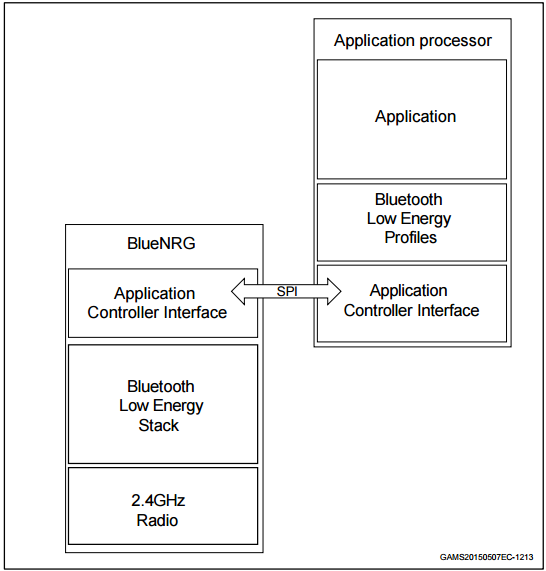
\includegraphics[width=3.5in, height=3in]{images/bluenrg_spi.png}
	\caption{BlueNRG SPI Interface}
\end{figure}
\subsubsection{Pin Description}
\begin{table}[ht]
	\centering
	\scalebox{0.5}{
	\begin{tabular}{|K{5cm} | K{5cm} | K{3cm} | K{2cm} | K{10cm}|}
		\toprule
		\rowcolor{Gray}
		\textbf{QFN32 pins} & \textbf{WLCSP pins}  & \textbf{Name} & \textbf{I/O} & \textbf{Description} \\
		\hline
		1 & E2 & SPI\_MOSI & I & SPI\_MOSI \\
		\hline
		2 & E1 & SPI\_CLK & I & SPI\_CLK \\
		\hline
		3 & D2 & SPI\_IRQ & O & SPI\_IRQ \\
		\hline
		4 & D1 & TEST1 & IO & Test pin \\
		\hline
		5 & C1 & VBAT3 & VDD & 2.0-3.6 battery voltage input \\
		\hline
		6 & C2 & TEST2 & IO & Test pin connected GND \\
		\hline
		7 & B1 & TEST3 & IO & Test pin connected GND \\
		\hline
		8 & B2 & TEST4 & IO & Test pin connected GND\\
		\hline
		9 & A1 & TEST5 & IO & Test pin connected GND\\
		\hline
		10 & B3 & TEST6 & IO & Test pin connected GND\\
		\hline
		11 & A2 & TEST7 & IO & Test pin connected GND\\
		\hline
		12 & A3 & VDD1V8 & O & 1.8 V digital core\\
		\hline
		13 & A4 & TEST8 & IO & Test pin not connected\\
		\hline
		14 & A5 & TEST9 & IO & Test pin not connected\\
		\hline
		15 & B4 & TEST11 & IO & Test pin not connected (QFN32), Test pin connected to GND (WLCSP)\\ 
		\hline
		16 & B5 & TEST12 & IO & Test pin not connected (QFN32), Test pin connected to GND (WLCSP) \\
		\hline
		17 & A6 & FXTAL1 & I & 16/32 MHz crystal\\
		\hline
		18 & B6 & FCTAL0 & I & 16/32 MHz crystal\\
	\bottomrule
	\end{tabular}}
	\caption{BlueNRG Pin Description part-I}
\end{table}
\begin{table}[ht]
	\centering
	\scalebox{0.5}{
	\begin{tabular}{|K{5cm} | K{5cm} | K{3cm} | K{2cm} | K{10cm}|}
		\toprule
		\rowcolor{Gray}
		\textbf{QFN32 pins} & \textbf{WLCSP pins}  & \textbf{Name} & \textbf{I/O} & \textbf{Description} \\
		19 & - & VBAT2 & VDD & 2.0-3.6 nattery voltage input\\
		\hline
		20 & C6 & RF1 & IO & Antenna + matching circuit\\
		\hline
		21 & D6 & RF0 & IO & Antenna + matching circuit\\
		\hline
		22 & E6 & SXTAL1 & I & 32 KHz crystal\\
		\hline
		23 & E5 & SXTAL0 & I & 32 KHz crystal\\
		\hline
		24 & D5 & VBAT1 & VDD & 2.0-3.6 battery voltage input\\
		\hline
		25 & E4 & RESETN & I & Reset\\
		\hline
		26 & F6 & SMPSFILT1 & O &  SMPS output\\
		\hline
		27 & - & NO\_SMPS & I & Power management strategy selection\\
		\hline
		28 & F5 & SMPSFILT2 & IO & SMPS input-ouput\\
		\hline
		29 & F3 & VDD1V2 & O & 1.2 V digital core\\
		\hline
		30 & E3 & TEST10 & IO & TEST pin connected to GND\\
		\hline
		31 & F2 & SPI\_CS & I & SPI\_CS\\
		\hline
		32 & F1 & SPI\_MISO & O & SPI\_MISO\\
		\hline
		- & C3 & GND & GND & Ground\\
		\hline
		- & D3 & GND & GND & Ground\\
		\hline
		- & D4 & GND & GND & Ground\\
		\hline
		- & F4 & SMPS-GND & GND & SMPS ground\\
	\bottomrule
	\end{tabular}}
	\caption{BlueNRG Pin Description part-II}
\end{table}
\subsubsection{Core, Memory and Peripherals}
The device contains an ARM Cortex-M0 microcontroller core that supports ultra-low leakage state retention mode and almost instantaneously returning to fully active mode on critical events. \\
The memory subsystem consists of 64 KB Flash, and 12 KB RAM , divided in two blocks of 6 KB (RAM1 and RAM2). Flash is used for the M0 program. No RAM or FLASH resources are available to the external microcontroller driving the BlueNRG.\\
The application controller interface (ACI) uses a standard SPI slave interface as transport layer, basing in five physical wires:
\begin{itemize}
	\item 2 control wires (clock and slave select) 
	\item 2 data wires with serial shift-out (MOSI and MISO) in full duplex 
	\item 1 wire to indicate data availability from the slave
\end{itemize}
\begin{table}[ht]
	\centering
	\scalebox{0.8}{
		\begin{tabular}{|c|c|c|c|}
			\toprule
			\rowcolor{Gray}
			\textbf{Name} & \textbf{Direction} &\textbf{Width} &\textbf{Description} \\
			\hline
			SPI\_CS & In & 1 & SPI slave select = SPI enable\\
			\hline
			SPI\_CCL & In & 1 & SPI clock (max 8MHz)\\
			\hline
			SPI\_MOSI & In & 1 & Master output, slave input\\
			\hline
			SPI\_MISO & Out & 1 & Master input, slave output\\
			\hline
			SPI\_IRQ & Out & 1 & Slave has data for master\\
			\bottomrule
		\end{tabular}
	}
	\caption{SPI Description}
\end{table}
All the SPI pins have an internal pull-down except for the CSN that has a pull-up. All the SPI pins, except the CSN, are in high impedance state during the low-power states. The IRQ pin needs a pull-down external resistor.
\subsubsection{Power Management}
The device integrates both a low dropout voltage regulator (LDO) and a step-down DC-DC converter, and one of them can be used to power the internal circuitry. However even when the LDO is used, the stringent maximum current requirements, which are advisable when coin cell batteries are used, can be met and further improvements can be obtained with the DC-DC converter at the sole additional cost of an inductor and a capacitor.
\subsubsection{Bluetooth Low Energy Radio}
The device integrates an RF transceiver compliant with the Bluetooth specification and the standard national regulations in the unlicensed 2.4 GHz ISM band. The RF transceiver requires very few external discrete components. It provides 96 dB link budgets with excellent link reliability, keeping the maximum peak current below 15 mA. In Transmit mode, the power amplifier (PA) drives the signal generated by the frequency synthesizer out to the antenna terminal through a very simple external network. The power delivered as well as the harmonic content depends on the external impedance seen by the PA.
\subsubsection{Operating Modes}
Several operating modes are defined for the BlueNRG:
\begin{itemize}
	\item Reset mode
	\item Sleep mode 
	\item Standby mode 
	\item Active mode 
	\item Radio mode 
	\begin{itemize}
		\item Receive Radio mode 
		\item Transmit Radio mode
	\end{itemize}
\end{itemize}
In Reset mode, the device is in ultra-low power consumption: all voltage regulators, clocks and the RF interface are not powered. The device enters Reset mode by asserting the external reset signal. As soon as it is de-asserted, the device follows the normal activation sequence to transit to Active mode. \\
In Sleep mode either the low speed crystal oscillator or the low speed ring oscillator are running, whereas the high speed oscillators are powered down as well as the RF interface. The state of the device is retained and the content of the RAM is preserved. Depending on the application, part of the RAM (RAM2 block) can be switched off during sleep to save more power (refer to stack mode 1, described in UM1868). \\
While in Sleep mode, the device waits until an internal timer expires and then it goes into Active mode. The transition from Sleep mode to Active mode can also be activated through the SPI interface. \\
Standby mode and Sleep mode are equivalent but the low speed frequency oscillators are powered down. In Standby mode the device can be activated through the SPI interface. \\
In Active mode the device is fully operational: all interfaces, including SPI and RF, are active as well as all internal power supplies together with the high speed frequency oscillator. The MCU core is also running. \\
Radio mode differs from Active mode as also the RF transceiver is active and it is capable of either transmitting or receiving.
\begin{figure}[ht]
	\centering
	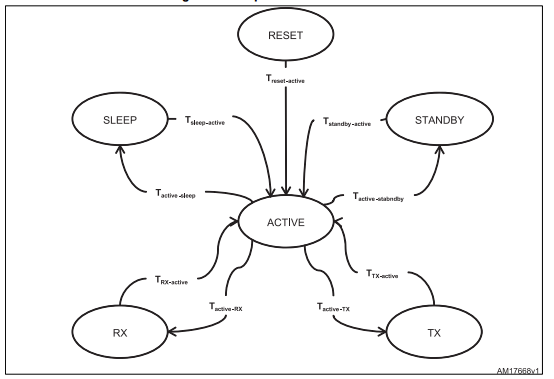
\includegraphics[width=3.5in, height=3in]{images/operating_modes.png}
	\caption{BlueNRG Operating Modes}
\end{figure}
\begin{table}[ht]
	\centering
	\scalebox{0.7}{
		\begin{tabular}{|K{2cm}| K{4cm} | K{2cm}|K{2cm}|K{2cm}|K{2cm}|K{2cm}|K{2cm}|K{2cm}|}
			\toprule
			\rowcolor{Gray}
			\textbf{State} & \textbf{Digital LDO} & \textbf{SPI} & \textbf{LSOSC} & \textbf{HSOSC} & \textbf{Core} & \textbf{RF synt.} & \textbf{RX chain} & \textbf{TX chain} \\
			\hline
			Reset & OFF Register contents lost & OFF & OFF & OFF & OFF & OFF & OFF & OFF \\
			\hline
			Standby & ON Register contents retained & ON & OFF & OFF & OFF & OFF & OFF & OFF \\
			\hline
			Sleep & ON Register contents retained & ON & ON & OFF & OFF & OFF & OFF & OFF \\
			\hline
			Active & ON Register contents retained & ON & . & ON & ON & OFF & OFF & OFF \\
			\hline
			RX & ON Register contents retained & ON & . & ON & ON & ON & ON & OFF \\
			\hline
			TX & ON Register contents retained & ON & . & ON & ON & ON & OFF & ON\\
			\bottomrule
		\end{tabular}
	}
	\caption{BlueNRG operating modes summary}
\end{table}
